\begin{figure}[p]
  \centering
  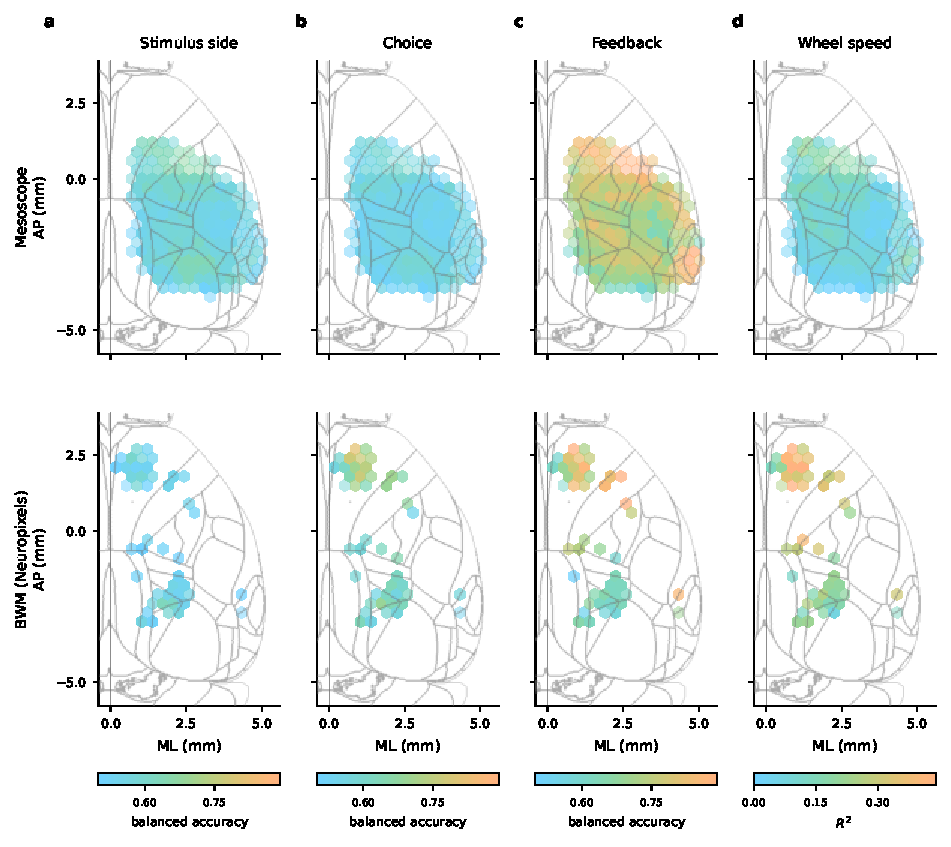
\includegraphics[width=7.00in,height=0.78\textheight,keepaspectratio]{si/si_strict_decoding_all_panels.pdf}
  \caption{Strict inclusion: only bins (0.4\,mm vertex to vertex, hemispheres folded) with $\geq$3 sessions from $\geq$2 animals, each session contributing $\geq$10 neurons. Isoluminant colour map; opacity encodes the number of animals (2: 50\,\%, 3: 75\,\%, $\geq$4: 100\,\%), so bins backed by few animals fade towards white. Mesoscope top row, BWM bottom row. Decoding from all neurons of the session in the bin, averaged across sessions; otherwise as in the main decoding figures. The binary variables share one colour scale. Mesoscope bins hold many more neurons than BWM bins, so the rows are not comparable in level. \textbf{a} Stimulus side. \textbf{b} Choice. \textbf{c} Feedback. \textbf{d} Wheel speed ($R^2$).}
  \label{fig:si_strict_decoding_all}
\end{figure}
